\section*{Math 202a - HW5 - Dan Davison - \texttt{ddavison@berkeley.edu}}

\begin{mdframed}
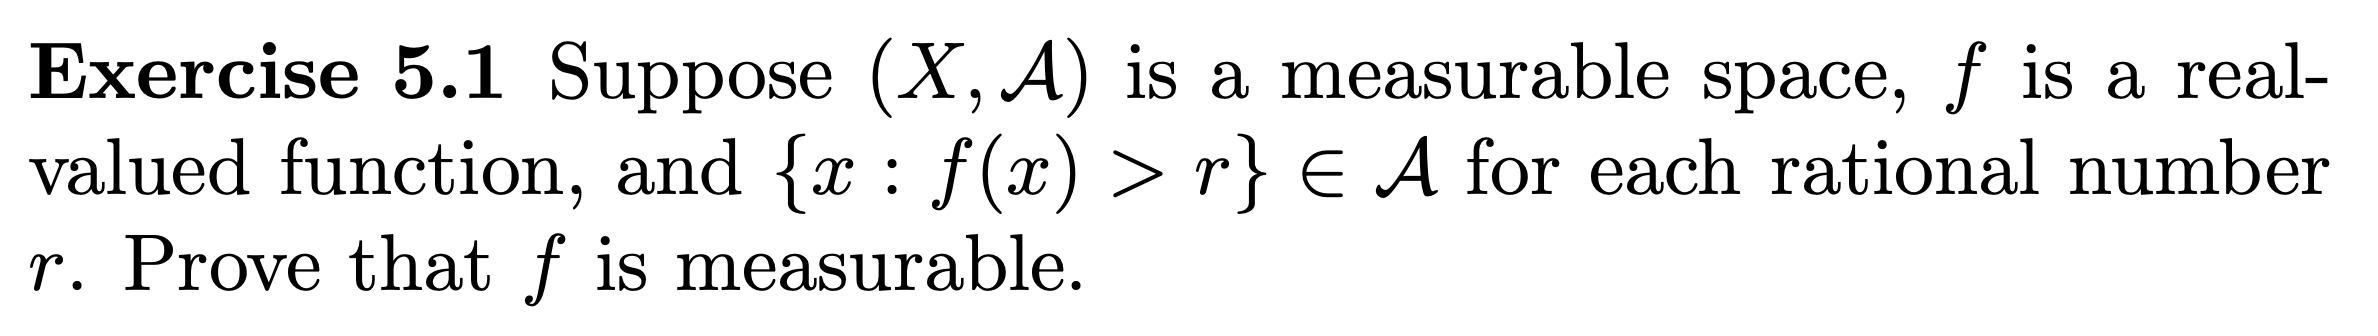
\includegraphics[width=400pt]{img/analysis--berkeley-202a-hw06-ab56.png}
\end{mdframed}

\begin{proof}
  Let $a \in \R$. Let $Q_{>a} = \{r ~:~ r \in \Q, r > a\}$. Since $Q_{>a} \subset \Q$, it is countable. Then
  \begin{align*}
    \{x ~:~ f(x) > a\} = \bigcup_{r \in Q_{>a}} \{x ~:~ f(x) > r\}.
  \end{align*}
  Therefore $\{x ~:~ f(x) > a\}$ is a countable union of elements of $\mc A$, for all $a \in \R$.

  \red{TODO} prove that the countable union is equal to the LHS. Use an explicit sequence of rationals? E.g. expansion
  of $a$ truncated at $n$-th digit.
\end{proof}



\newpage
\begin{mdframed}
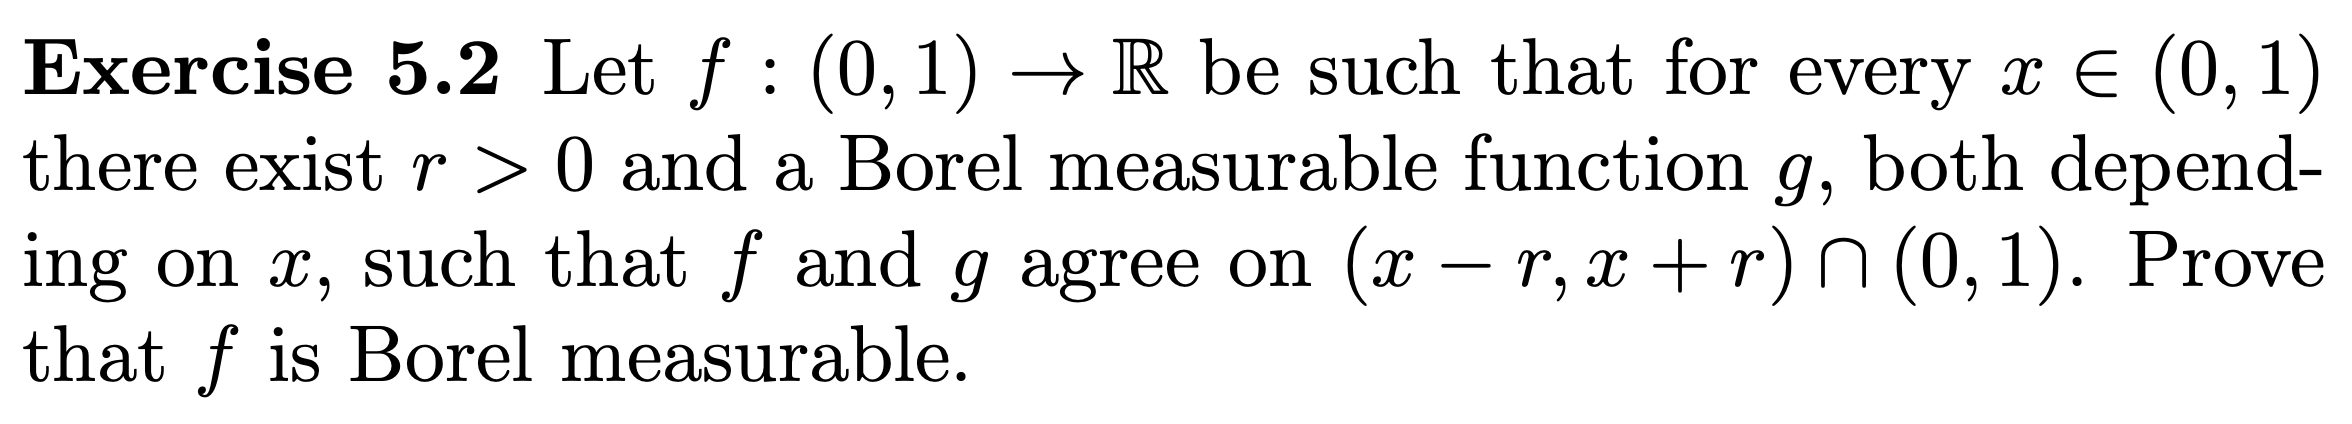
\includegraphics[width=400pt]{img/analysis--berkeley-202a-hw06-927a.png}
\end{mdframed}

\begin{proof}
  Let $\mc A$ be the Borel $\sigma$-algebra on $(0, 1)$ and for every $x \in (0, 1)$ let $r_x > 0$ be such
  that $f$ and $g_x$ agree on $(x - r_x, x + r_x) \cap (0, 1)$, and $g_x$ is Borel-measurable.

  We must show that $\{x ~:~ f(x) > y\} \in \mc A$ for all $y \in \R$.

  Let $y \in \R$ and let $q_1, q_2, \ldots \in \Q \cap (0, 1)$ be an enumeration of the rationals in $(0, 1)$.

  Define $U_{a} := \{x ~:~ g_{a}(x) > y\} \cap (a - r_{a}, a + r_{a})$. Note that $U_a$ is a set of real
  numbers $x$ near $a$ for which we know that $f(x) > y$.

  We claim that $\{x ~:~ f(x) > y\} = \bigcup_{i=1}^\infty U_{q_i} \in \mc A$.

  Let $w = \inf \{r_{q_i} ~:~ i \in \N \}$.

  To prove the forwards inclusion, let $b \in \{x ~:~ f(x) > y\}$, and let $q \in (b - w, b + w) \cap \Q$. Note
  that $b \in (q - r_q, q + r_q)$ and therefore $g_q(b) = f(b) > y$. Therefore $b \in U_q$, proving the
  forwards inclusion.

  To prove the reverse inclusion, let $b \in \bigcup_{i=1}^\infty U_{q_i}$. Then $b \in U_q$ for
  some $q \in \{q_1, q_2, \ldots\}$. Therefore $f(b) > y$.

  Finally, note that $U_a$ is the intersection of two Borel-measurable sets and hence is Borel-measurable.
  Therefore $\bigcup_{i=1}^\infty U_{q_i}$ is Borel-measurable.
\end{proof}



\newpage
\begin{mdframed}
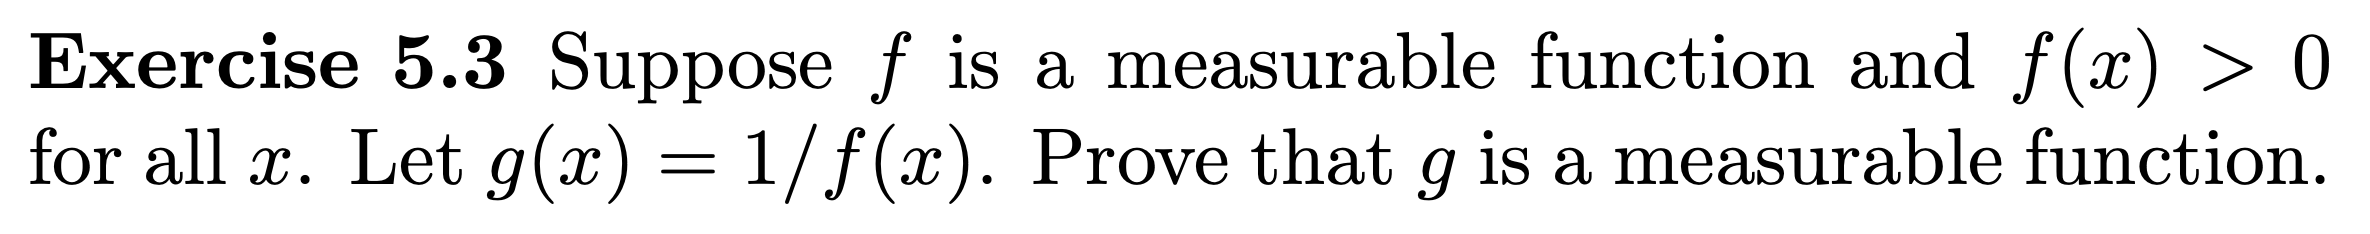
\includegraphics[width=400pt]{img/analysis--berkeley-202a-hw06-b799.png}
\end{mdframed}

\begin{lemma*}[A continuous function is measurable]\label{lemma-continuous-function-is-measurable}
  Let $Y \subseteq \R$ and let $g: X \to Y$ be a continuous function.

  We must show that there exists a $\sigma$-algebra such that $\{x ~:~ g(x) > y\} \in \mc A$ for all $y \in Y$.

  Let $y \in Y$ and let $U = g^{-1}((y, \infty))$. Then $U$ is open in $X$ since it is the preimage of an open
  set under a continuous function. Therefore $U$ is in the Borel $\sigma$-algebra on $X$.

  Therefore the Borel $\sigma$-algebra satisfies our requirement and $g$ is measurable.
\end{lemma*}


\begin{proof}
  Let $f: X \to (0, \infty)$ be a measurable function, and let $g(x) = 1/f(x)$.

  Since $f$ is measurable, there exists a $\sigma$-algebra $\mc A$ such that $f^{-1}((y, \infty)) \in \mc A$
  for all $y > 0$.

  Let $h(x) = 1/x$. Then $g = h \circ f$.

  Fix $y' \in (0, \infty)$ and let $U = h^{-1}((y', \infty)) \subseteq (0, \infty)$. Since $h$ is
  continuous, $U$ is open.

  We want to show that $g^{-1}((y', \infty)) \in \mc A$. We have
  \begin{align*}
    g^{-1}((y', \infty)) = f^{-1}(h^{-1}((y', \infty))) = f^{-1}(U).
  \end{align*}
  So what we want to show is that $f^{-1}(U) \in \mc A$, where $U \subseteq (0, \infty)$ is open.

  Write $U = \bigcup_{i=1}^\infty (a_i, b_i)$ where $(a_1, b_1), (a_2, b_2), \ldots \subseteq (0, \infty)$ is a
  countable pairwise disjoint collection of open intervals.

  Note that $f^{-1}(U) = \bigcup_{i=1}^\infty f^{-1}((a_i, b_i))$.

  Note also that $(a, b) = (a, \infty) \setminus (b, \infty)$ and therefore
  that $f^{-1}((a, b)) = f^{-1}((a, \infty)) \setminus f^{-1}((b, \infty))$.

  Thus we have
  \begin{align*}
    f^{-1}(U)
    &= \bigcup_{i=1}^\infty \Big(f^{-1}((a, \infty)) \setminus f^{-1}((b, \infty))\Big) \\
    &= \bigcup_{i=1}^\infty \Big(f^{-1}((a, \infty)) \cap \big(f^{-1}((b, \infty))\big)^c\Big) \\
    &\in \mc A.
  \end{align*}
\end{proof}


\newpage
\begin{mdframed}
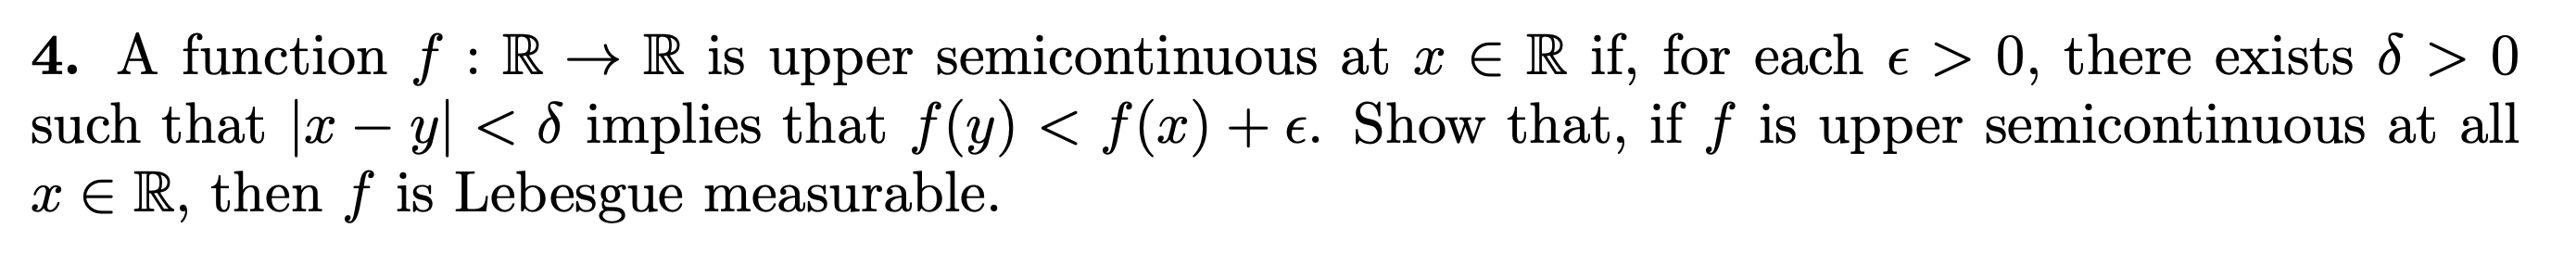
\includegraphics[width=400pt]{img/analysis--berkeley-202a-hw06-90b1.png}
\end{mdframed}




\begin{proof}
  It suffices to show that $\{x ~:~ f(x) < y\}$ is open for all $y \in \R$, since then $\{x ~:~ f(x) < y\}$ is
  Borel-measurable.

  Equivalently, it suffices to show that $f^{-1}\((-\infty, y)\)$ is open for all $y \in \R$.

  We have:

  For every $x \in \R$, for every $\eps > 0$ there exists $\delta$ such that $f((x - \delta, x + \delta)) \subseteq (-\infty, f(x) + \eps)$.

  We know that there is a theorem concerning continuous functions: $f:\R \to \R$ is continuous if and only
  if $f^{-1}(U)$ is open for every open subset $U \subseteq \R$.

  We want to prove the reverse direction of this, but assuming upper semicontinuity only. In other words, we
  want to prove that (upper semicontinuity) implies (preimage of $(-\infty, q)$ is open) for all $q \in \R$.

  So, let's follow the proof of the standard continuity theorem and see if we get into trouble.

  Let $B(x, r)$ denote the open interval $(x - r, x + r)$.

  Let $a \in \R$. Fix $\eps > 0$.

  Since $f$ is upper semicontinuous there exists $\delta > 0$ such
  that $(a - \delta, a + \delta) \subseteq f^{-1}\((-\infty, f(a) + \eps)\)$.
  Therefore $f^{-1}\((-\infty, f(a) + \eps)\)$ is a neighborhood of $a$.

  What we want to conclude is that $f^{-1}\((-\infty, y)\)$ is open for all $y \in \R$.

\end{proof}



\begin{theorem*}[Preimage of an open set under a continuous function is open]
  $f:\R \to \R$ is continuous if and only if $f^{-1}(U)$ is open for every open subset $U \subseteq \R$.
\end{theorem*}

\begin{proof}
  First we prove that continuity implies open preimages.

  Let $B(x, r)$ denote the open interval $(x - r, x + r)$.

  Let $a \in \R$ and suppose $f$ is continuous at $a$. Fix $\eps > 0$.

  Since $f$ is continuous there exists $\delta > 0$ such
  that $B(a,  \delta) \subseteq f^{-1}(B(f(a), \eps))$. Therefore $f^{-1}(B(f(a), \eps))$ is a
  neighborhood of $a$.

  Since by hypothesis $f$ is continuous at all $a \in \R$, we have that $f^{-1}(U)$ is a neighborhood of all of
  its points. This is because:

  Let $x \in f^{-1}(U)$. Then $f(x) \in U$. Since $U$ is open there exists $\eps$ such
  that $B(f(x), \eps) \subseteq U$ and $\delta$ such that $B(x, \delta) \subseteq B(f(x), \eps)$ is a
  neighborhood of $x$.
\end{proof}
\newpage
\begin{mdframed}
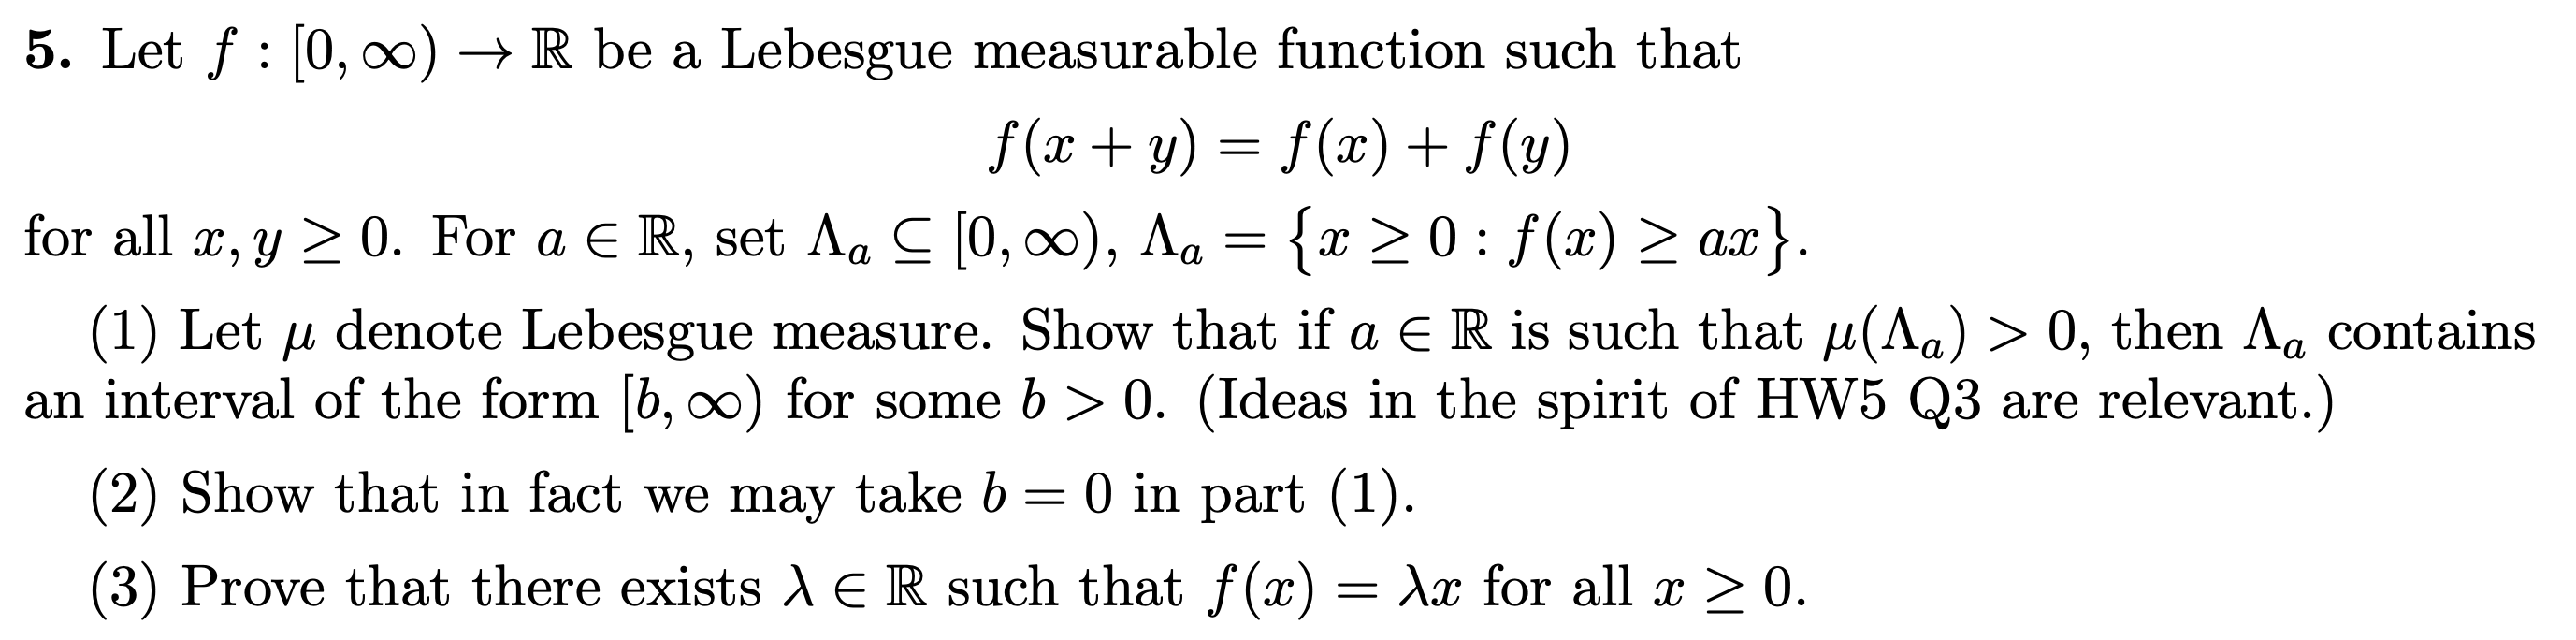
\includegraphics[width=400pt]{img/analysis--berkeley-202a-hw06-7769.png}
\end{mdframed}


\newpage
\begin{mdframed}
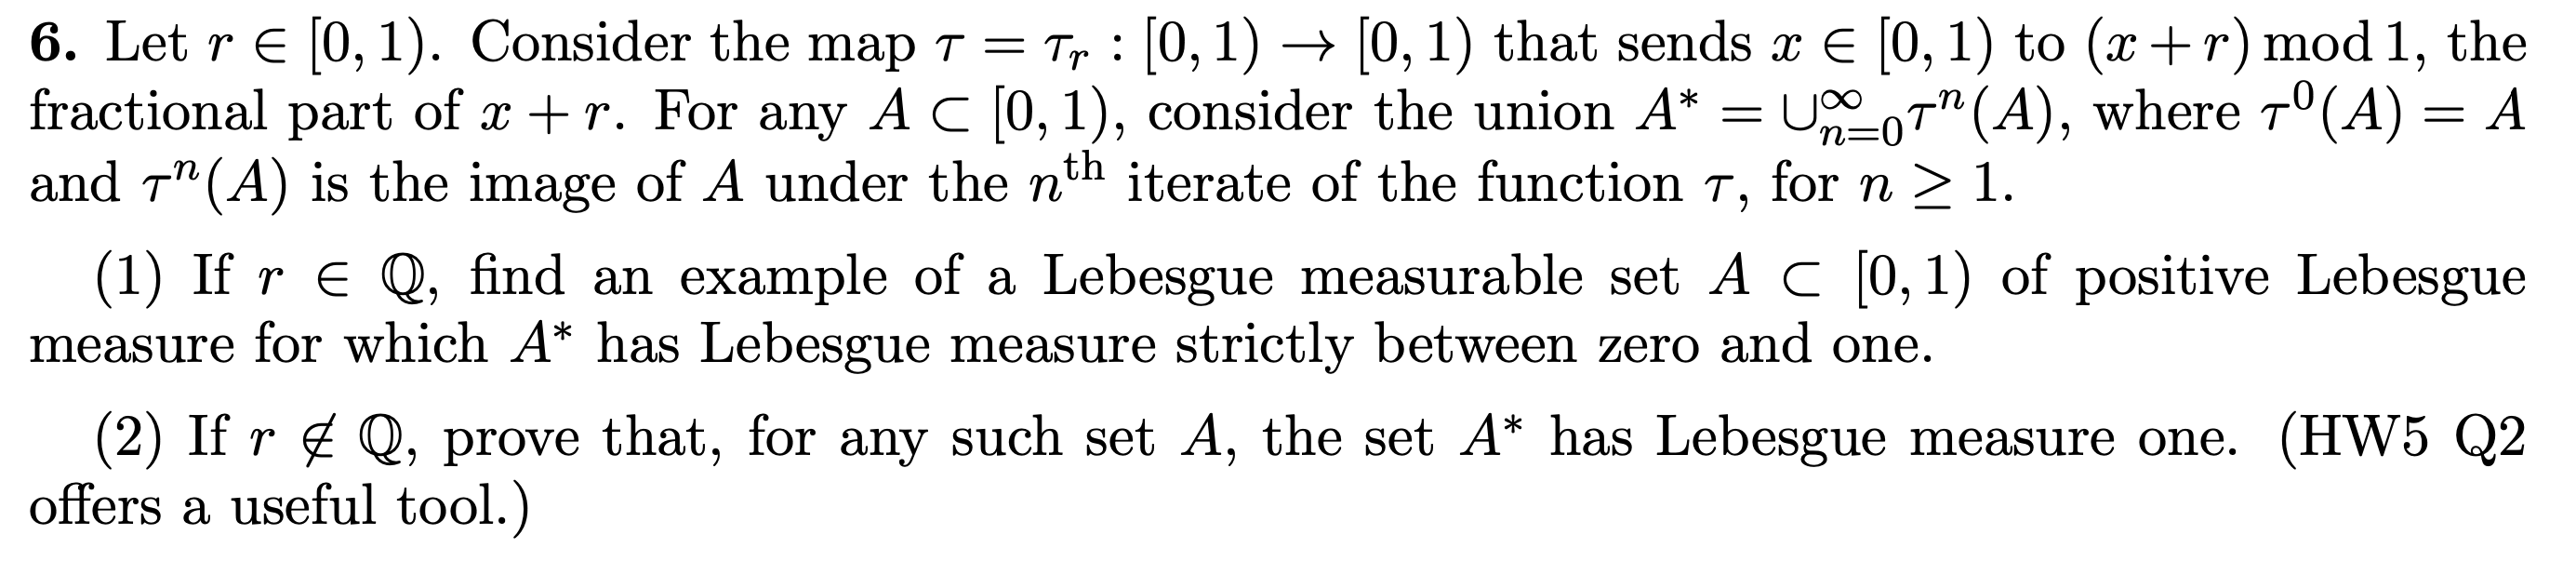
\includegraphics[width=400pt]{img/analysis--berkeley-202a-hw06-9bc5.png}
\end{mdframed}